\documentclass[usenames,dvipsnames]{beamer}
\usepackage[utf8]{inputenc}
\usepackage{verbatim}
\usetheme{umu}

\usepackage{enumitem}
\usepackage{siunitx}
\usepackage{xcolor}

%%% Bibliography
\usepackage[style=authoryear,backend=biber]{biblatex}
\addbibresource{bibliography.bib}

% Author names in publication list are consistent 
% i.e. name1 surname1, name2 surname2
% See https://tex.stackexchange.com/questions/106914/biblatex-does-not-reverse-the-first-and-last-names-of-the-second-author
\DeclareNameAlias{author}{first-last}

%%% Suppress biblatex annoying warning
\usepackage{silence}	
\WarningFilter{biblatex}{Patching footnotes failed}

%%% Some useful commands
% pdf-friendly newline in links
\newcommand{\pdfnewline}{\texorpdfstring{\newline}{ }} 
% Fill the vertical space in a slide (to put text at the bottom)
\newcommand{\framefill}{\vskip0pt plus 1filll}
\setbeamertemplate{caption}{\raggedright\insertcaption\par}

%%%%%%%%%%%%%%%%%%%%%%%%%%%%%%%%%%%%%%%%%%%%%%%%%%%%%%%%%%%%%%%%%%%%%%%%%%%%%%%%%%%%%
%%%%%%%%%%%%%%%%%%%%%%%%%%%%%%% YOUR PRESENTATION BELOW %%%%%%%%%%%%%%%%%%%%%%%%%%%%%
%%%%%%%%%%%%%%%%%%%%%%%%%%%%%%%%%%%%%%%%%%%%%%%%%%%%%%%%%%%%%%%%%%%%%%%%%%%%%%%%%%%%%
\title{Evolution of galaxy dynamics over the last 10 Gyrs with MUSE/VLT}
\date[\today]{\small\today}
\author[Mercier Wilfried]{
  \textbf{Author}: \hspace{33pt} Mercier Wilfried
  \pdfnewline
  \textbf{Supervisor}: \hspace{14pt} CONTINI Thierry
  \pdfnewline
  \textbf{Co-Supervisor}: Epinat Benoit
  }


\institute{Observatoire de Paris}

\begin{document}

\begin{frame}
\titlepage
\end{frame}


\section{IFS \& MUSE}
\begin{frame}{Integral Field Spectroscopy \& MUSE}

	\begin{columns}[T]
	
		\begin{column}{0.4\linewidth}
			\underline{IFS:}
			\begin{itemize}[label=$\rhd$]
				\item 3D cubes (2D spatial + 1D spectral)
				\item photometry + kinematics
			\end{itemize}					
		
		
			\underline{MUSE:}
			\begin{itemize}[label=$\rhd$]
				\item $1 \times \SI{1}{arcmin\squared}$ FoV
				\item $\SI{0.2}{arcsec}$ spatial sampling
				\item spectral range $[\SI{4650}{\angstrom}, \SI{9300}{\angstrom}]$
				\item seeing or AO observations
			\end{itemize}
		\end{column}

		\begin{column}{0.6\linewidth}
			\begin{figure}
				\vspace{-15pt}
				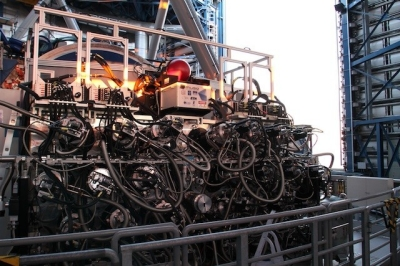
\includegraphics[width=\linewidth]{{graphics/MUSE}.jpg}
				\caption{MUSE instrument. Credit: Ghaouti Hansali (CRAL)}
			\end{figure}
		\end{column}
	\end{columns}

\end{frame}


\section{Initial sample}
\begin{frame}{Our sample}
	\begin{columns}
		\begin{column}{0.5\linewidth}	
			\begin{figure}
				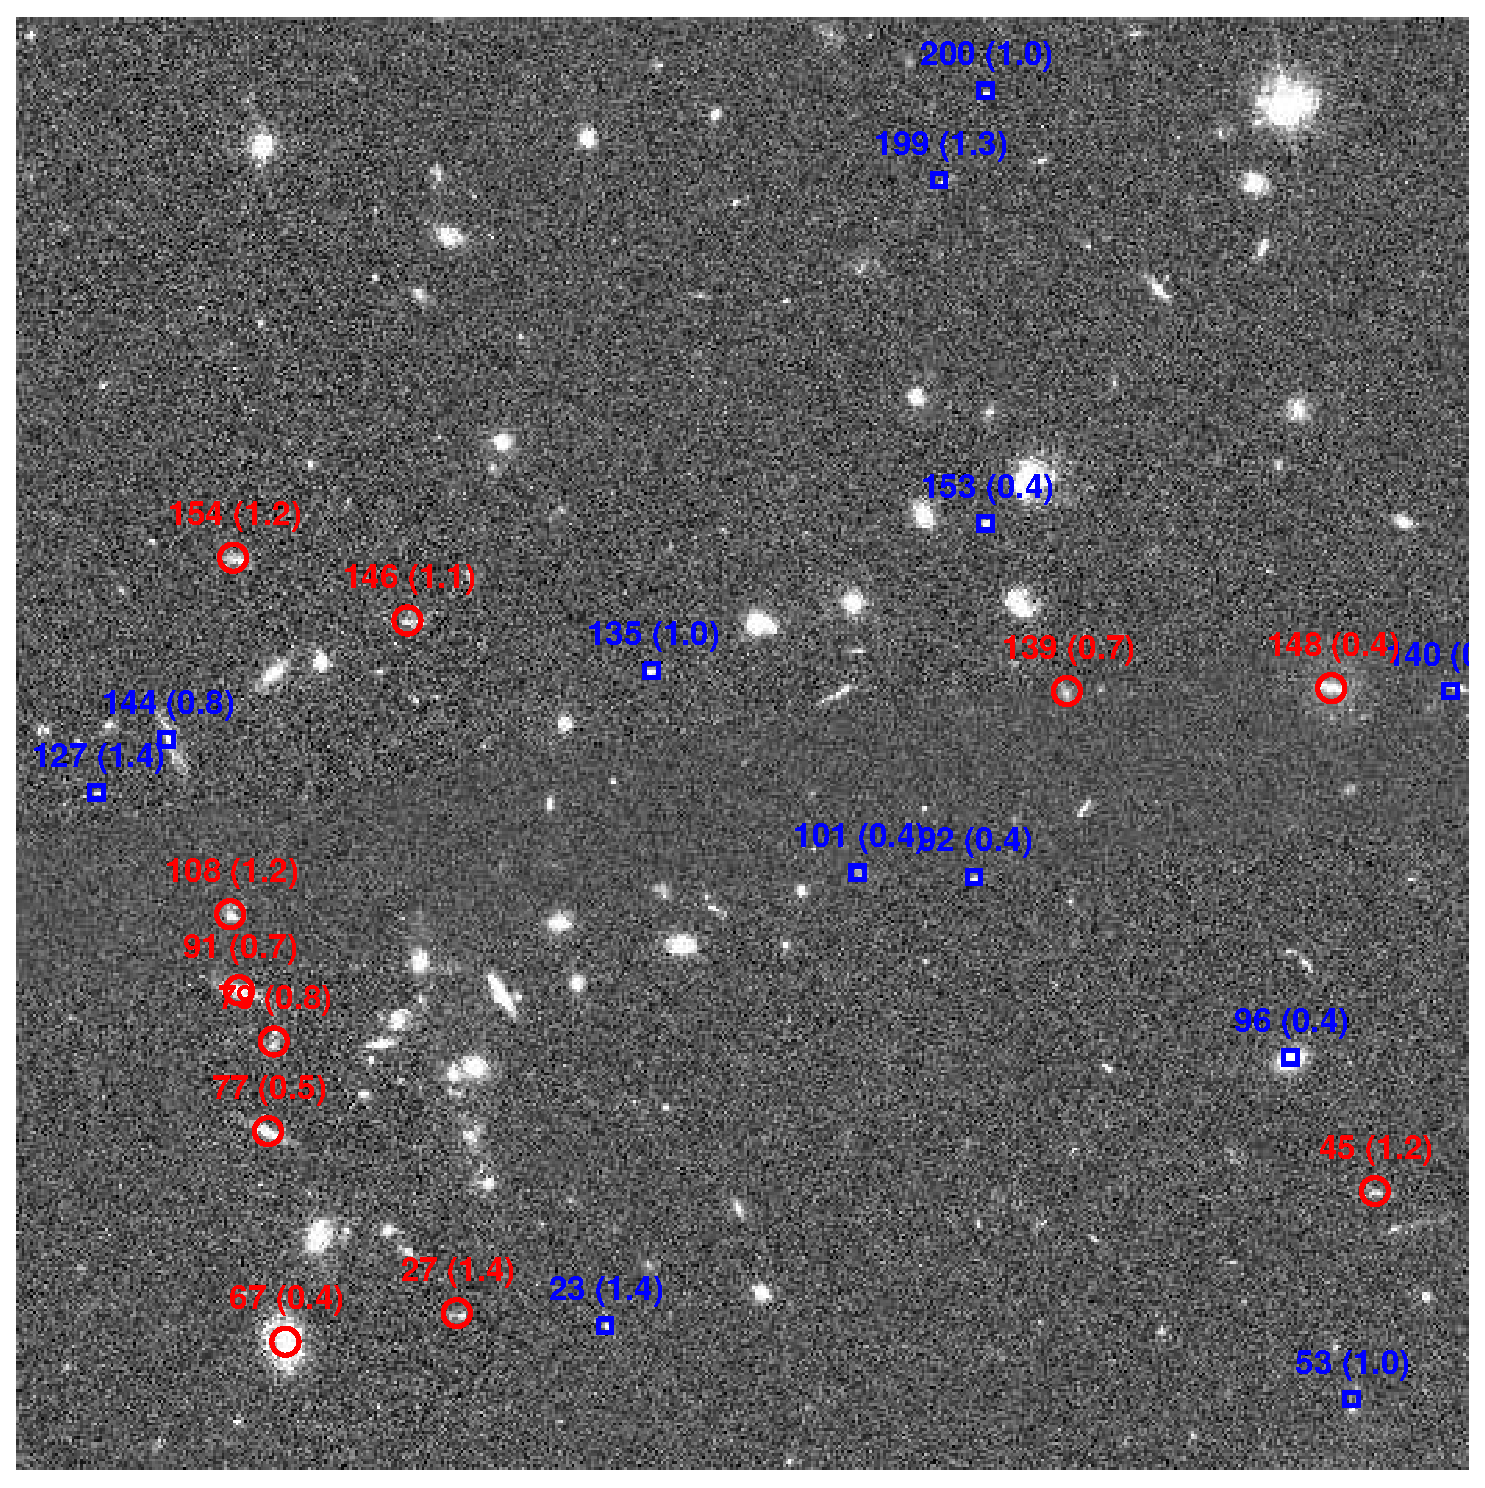
\includegraphics[width=\linewidth]{{graphics/CGr30}.eps}
				\caption{HST image of MUSE group CGr30}
			\end{figure}
		\end{column}
		
		\begin{column}{0.5\linewidth}
			\begin{itemize}[label=$\rhd$]
				\item $16$ MUSE fields in COSMOS area
				\begin{itemize}[label=$\cdot$]
					\item \textit{deep} and \textit{best\_seeing} observations
					\item CGr32 split in $3$ parts
				\end{itemize}
				\item $\sim 500$ field galaxies with [OII] detection
				\begin{itemize}[label=$\cdot$]
					\item HST-ACS counterparts
					\item $0.4 \leq z \leq 1.4$
				\end{itemize}
			\end{itemize}
		\end{column}
	\end{columns}
\end{frame}


\section{Checking a few parameters}
\subsection{Half-light Radius}
\begin{frame}{Checking a couple of parameters}
	\framesubtitle{Half-light radius}
	
	\begin{figure}
		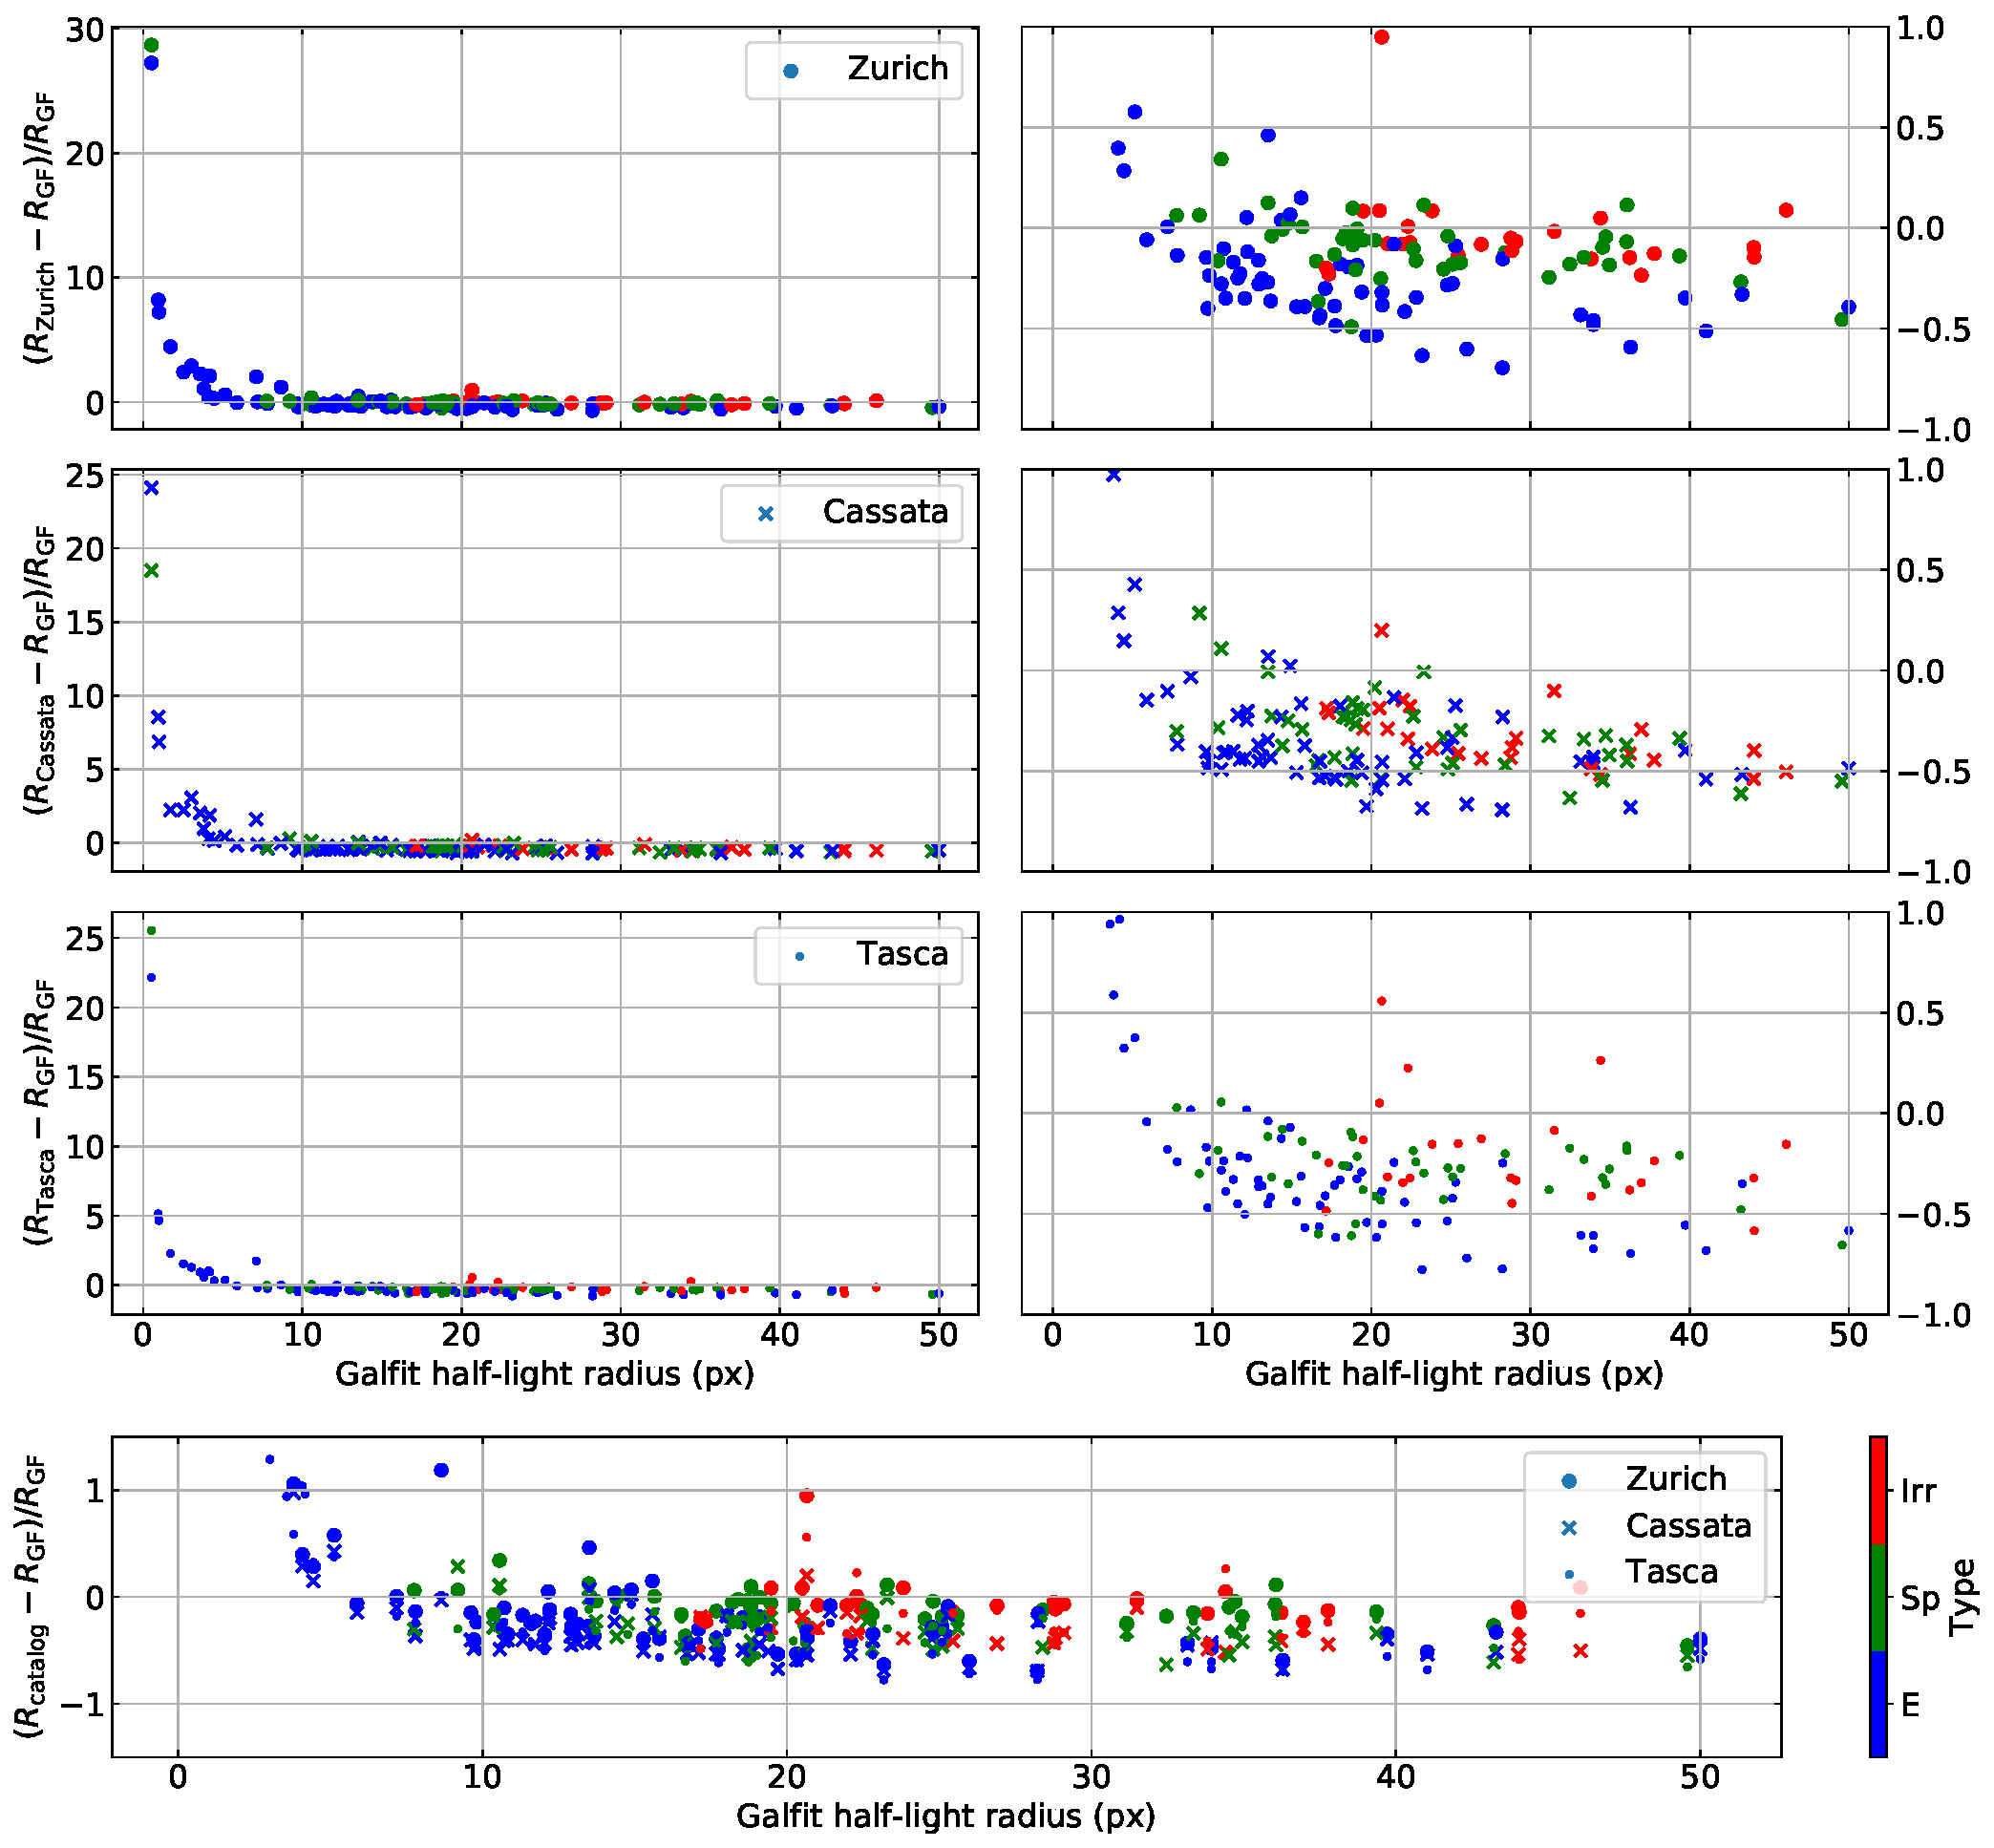
\includegraphics[width=0.85\linewidth]{{graphics/relErr_against_GalFit1.5LightRadius_colourCoded_CassataType}.pdf}
		\caption{spheroidal  \textcolor{OliveGreen}{disk-like}    \textcolor{magenta}{irregulars}}
	\end{figure}

\end{frame}


\subsection{Ellipticity}
\begin{frame}{Checking a few parameters}
	\framesubtitle{Ellipticity}
	\begin{columns}	
		\begin{column}{0.5\linewidth}
			\vspace{-10pt}		
			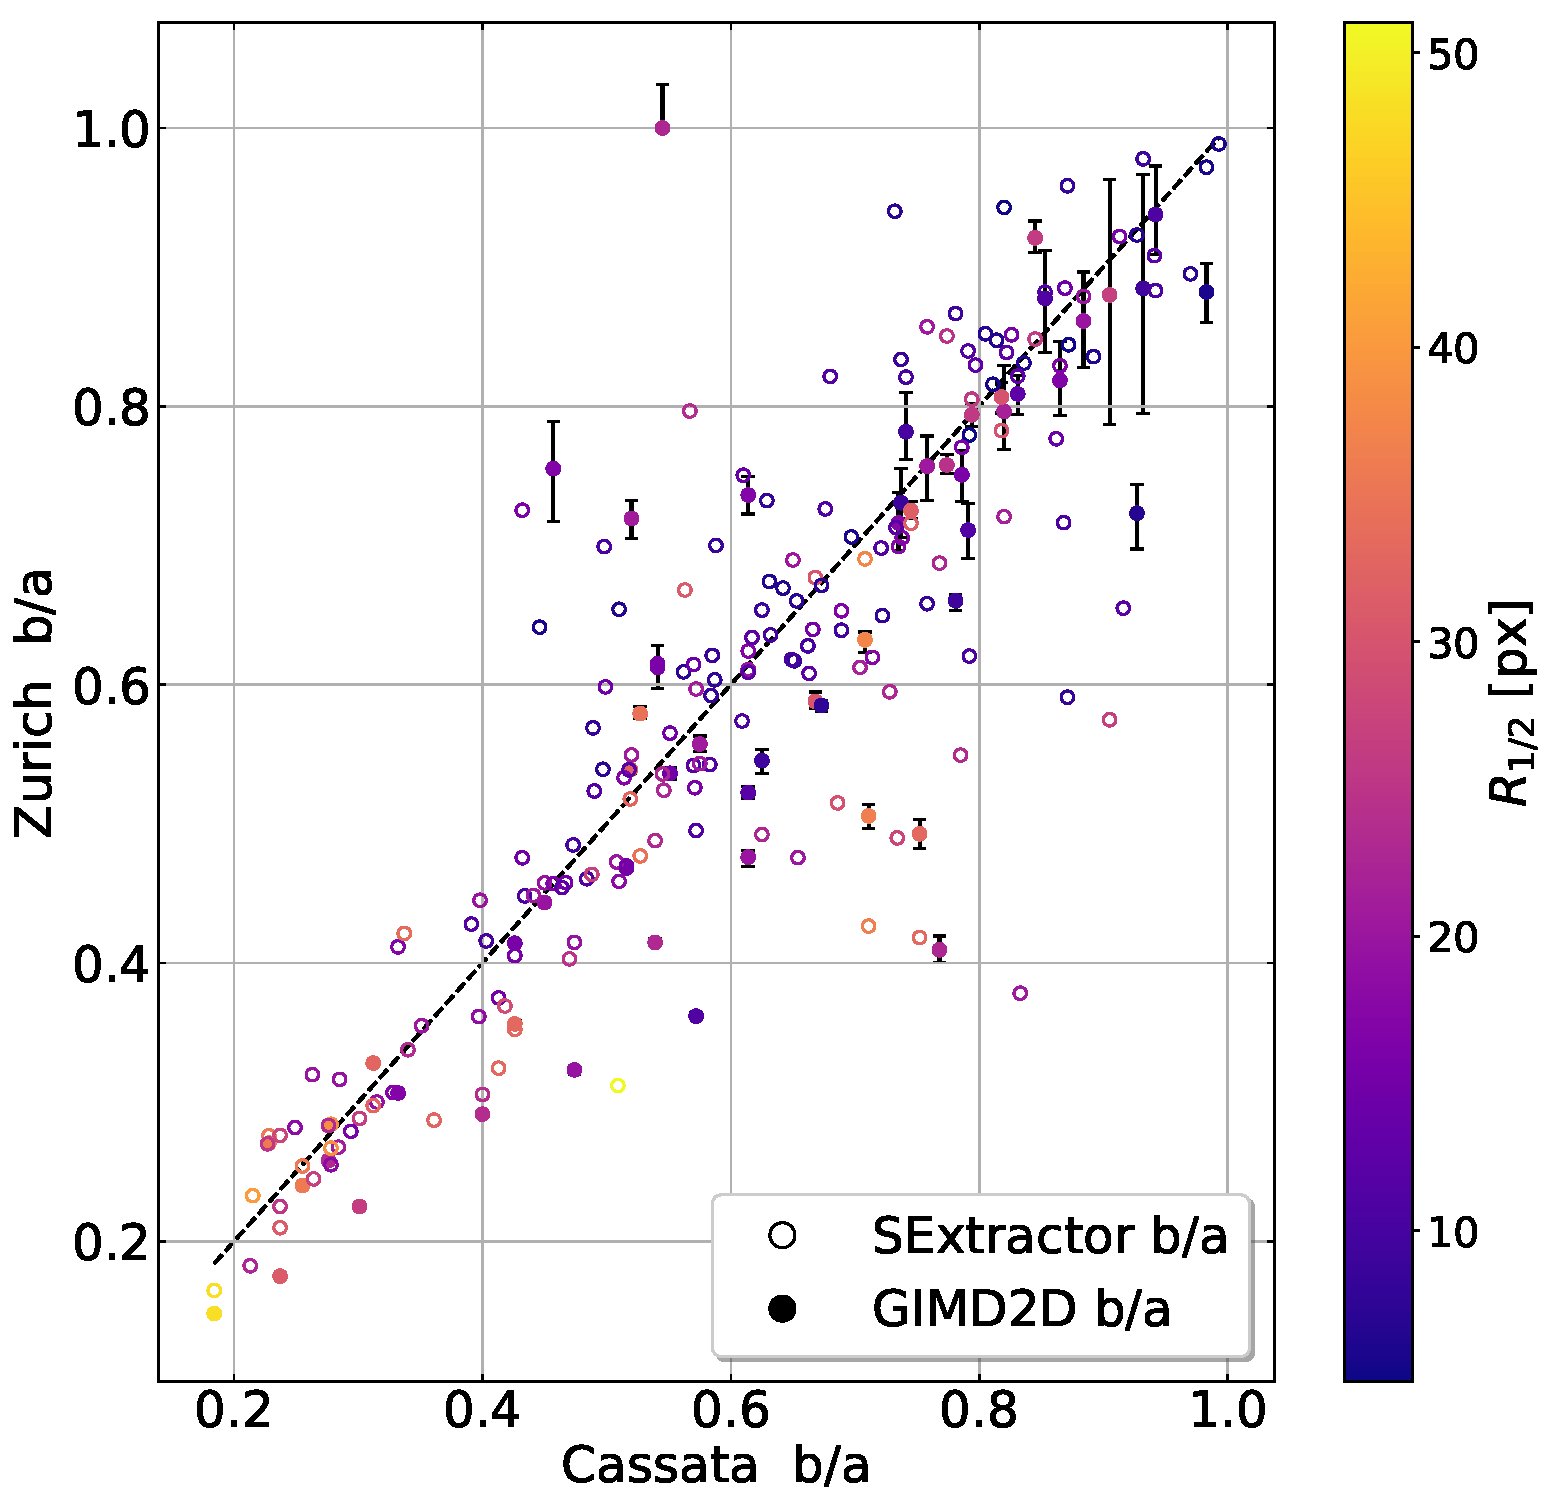
\includegraphics[width=\linewidth]{{graphics/check_b_a}.pdf}
			
			\begin{itemize}[label=$\rhd$]				
				\item values are consistent between catalogues
			\end{itemize}
		\end{column}
		
		\begin{column}{0.5\linewidth}
			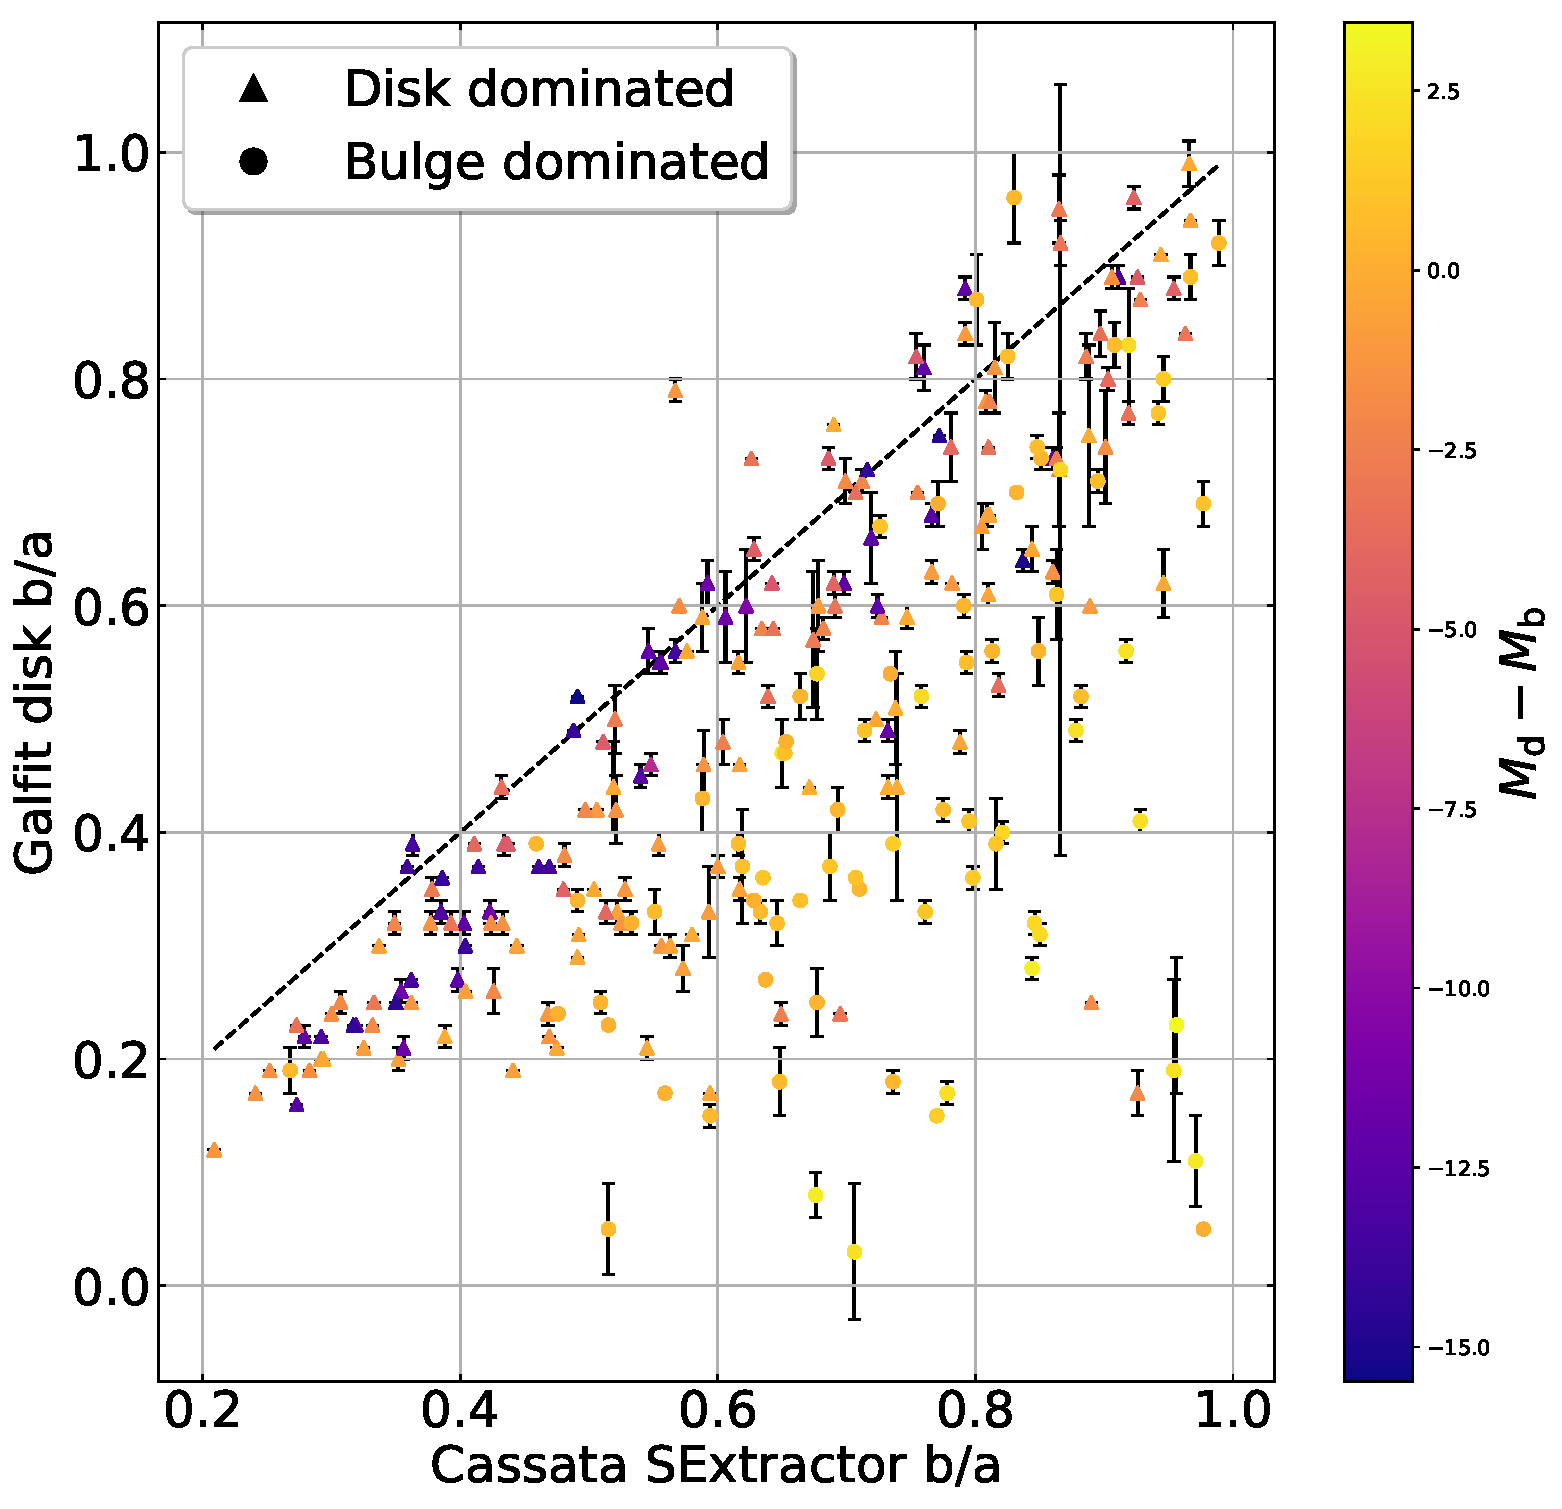
\includegraphics[width=\linewidth]{{graphics/check_b_a_GF}.pdf}
			
			\begin{itemize}[label=$\rhd$]				
				\item scatter is due to bulge dominated (spherically symmetric) systems
			\end{itemize}
		\end{column}
	\end{columns}
\end{frame}


\section{Characteristics of our sample}
\subsection{Redshift distribution}
\begin{frame}{Characteristics of our sample}
	\framesubtitle{Redshift distribution}
	\begin{columns}	
		\begin{column}{0.5\linewidth}
			\vspace{-10pt}		
			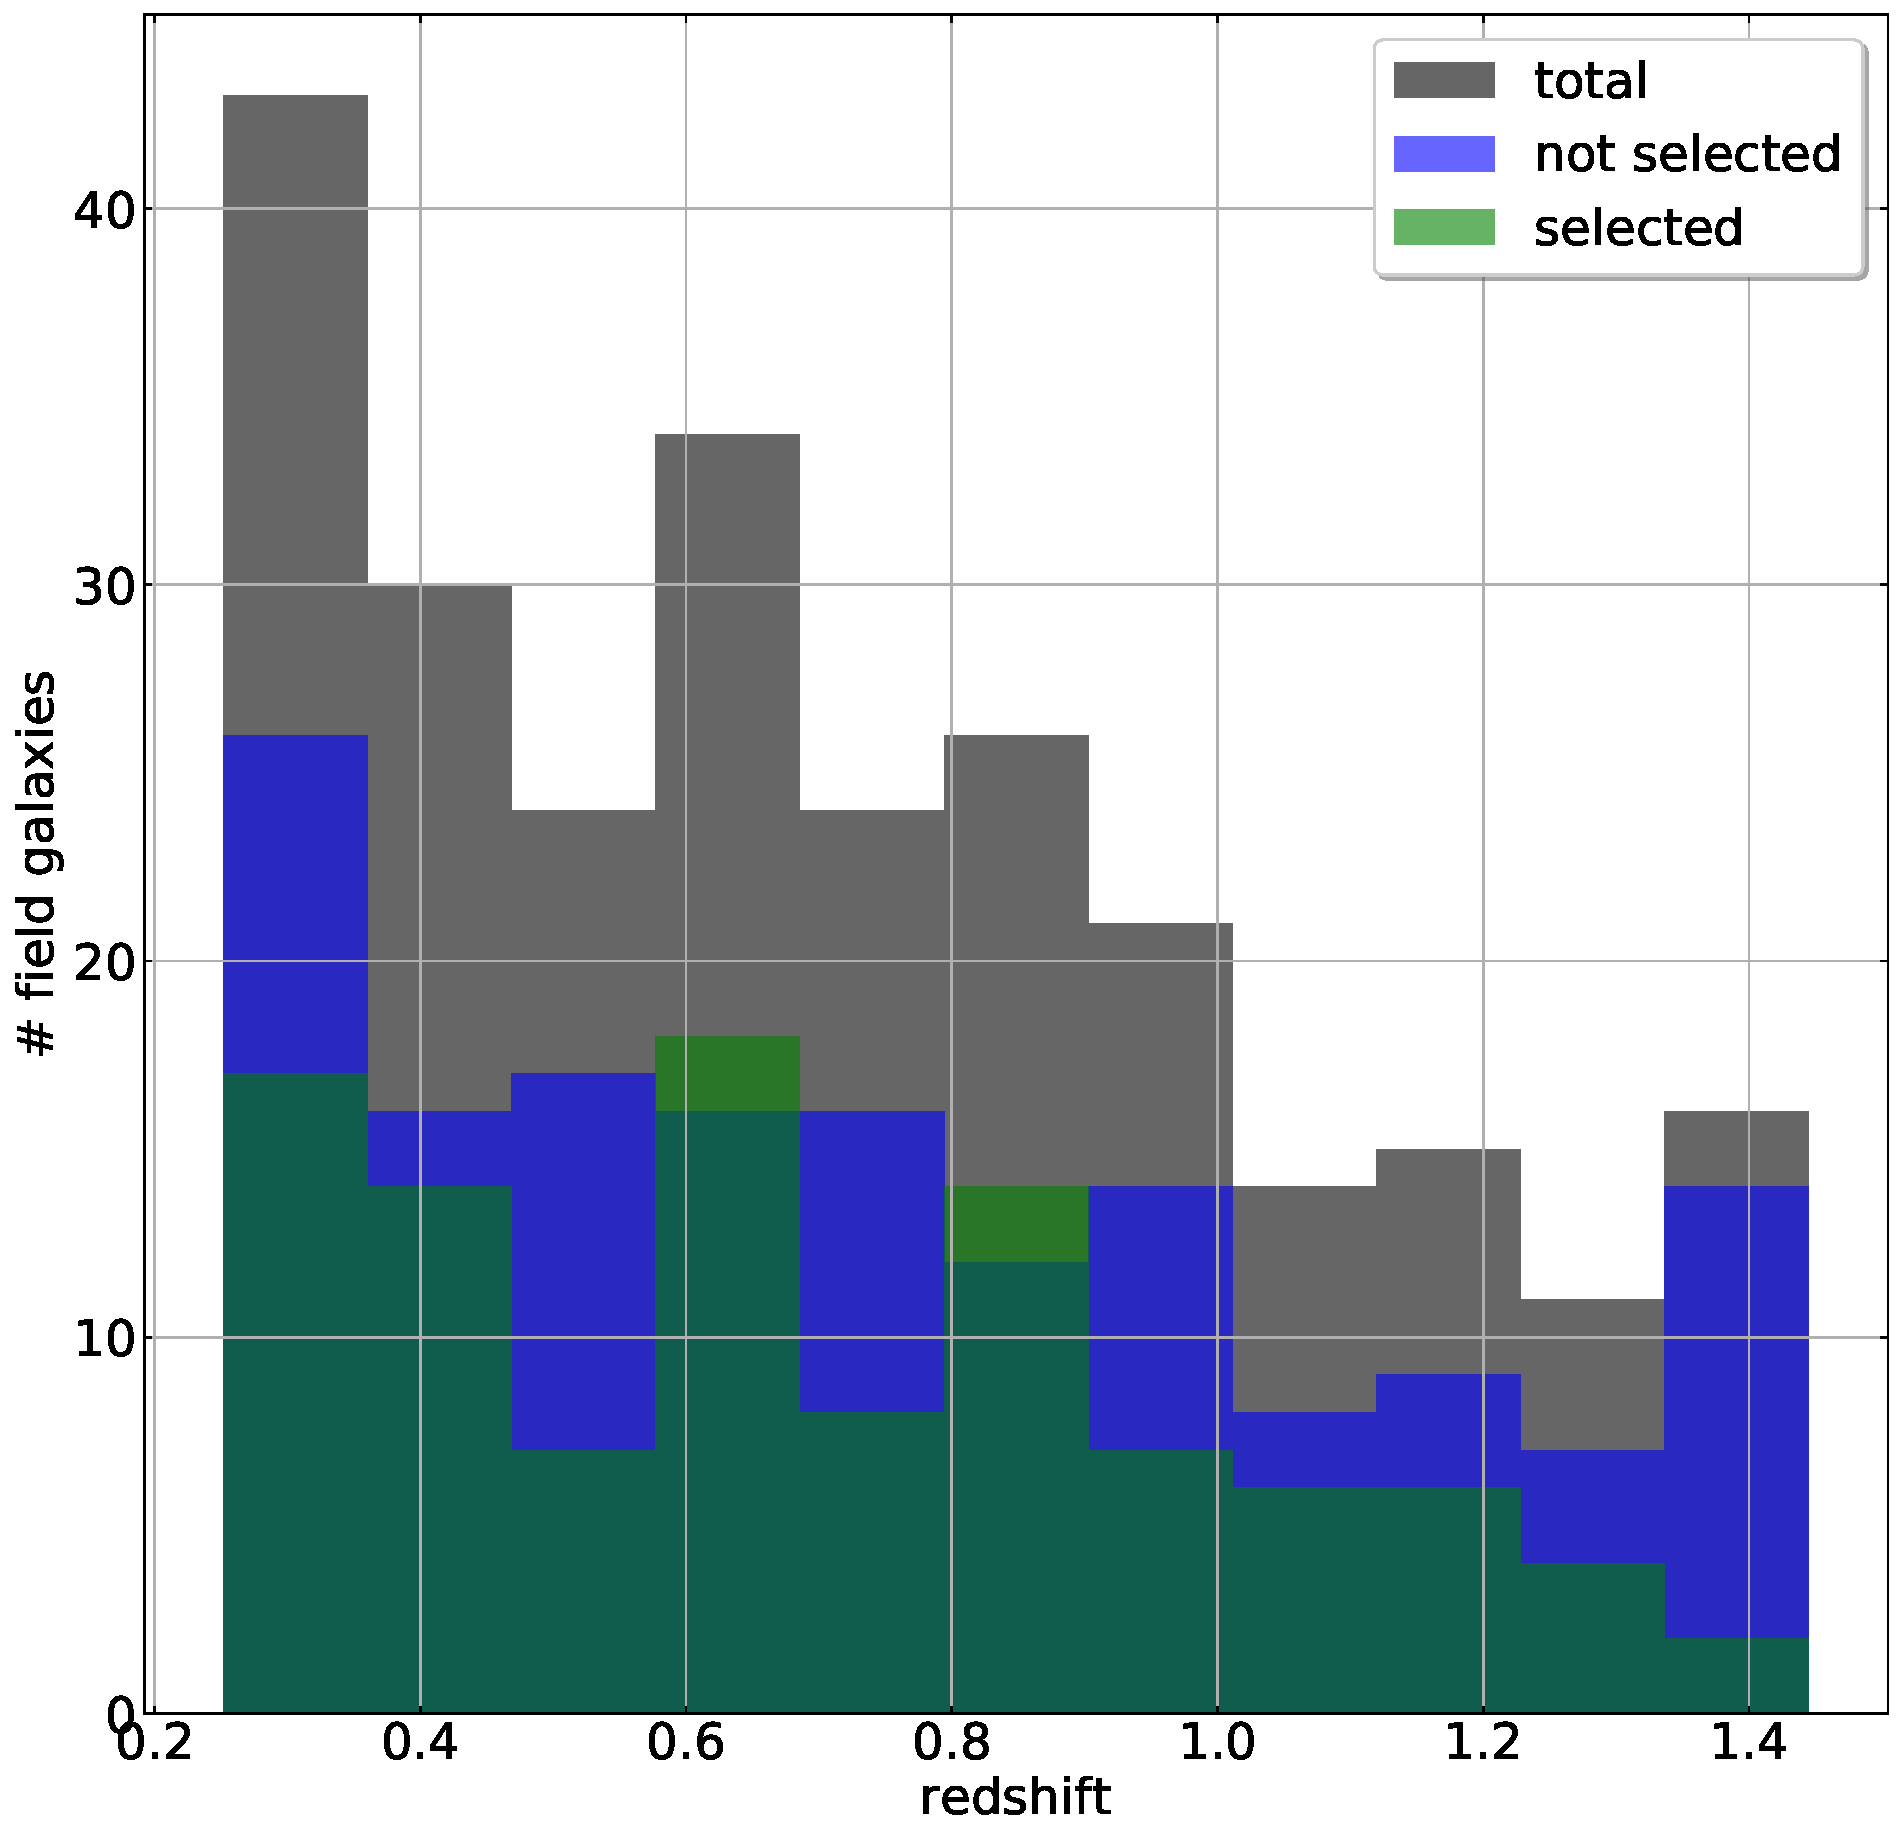
\includegraphics[width=\linewidth]{{graphics/hist_redshift}.pdf}
		\end{column}
		
		\begin{column}{0.5\linewidth}
			\begin{itemize}[label=$\rhd$]				
				\item sample of \textbf{103 galaxies} with $R_{\rm{1/2}} > \SI{0.35}{"}$ and $\rm{SNR} > 5$
				\item we loose galaxies at $z \approx 1.4$
				\item redshift distribution is not drastically changed
			\end{itemize}
		\end{column}
	\end{columns}

\end{frame}

\subsection{Mass-SFR relation}
\begin{frame}{Characteristics of our sample}
	\framesubtitle{Mass-SFR relation}
	\vspace{-3pt}
	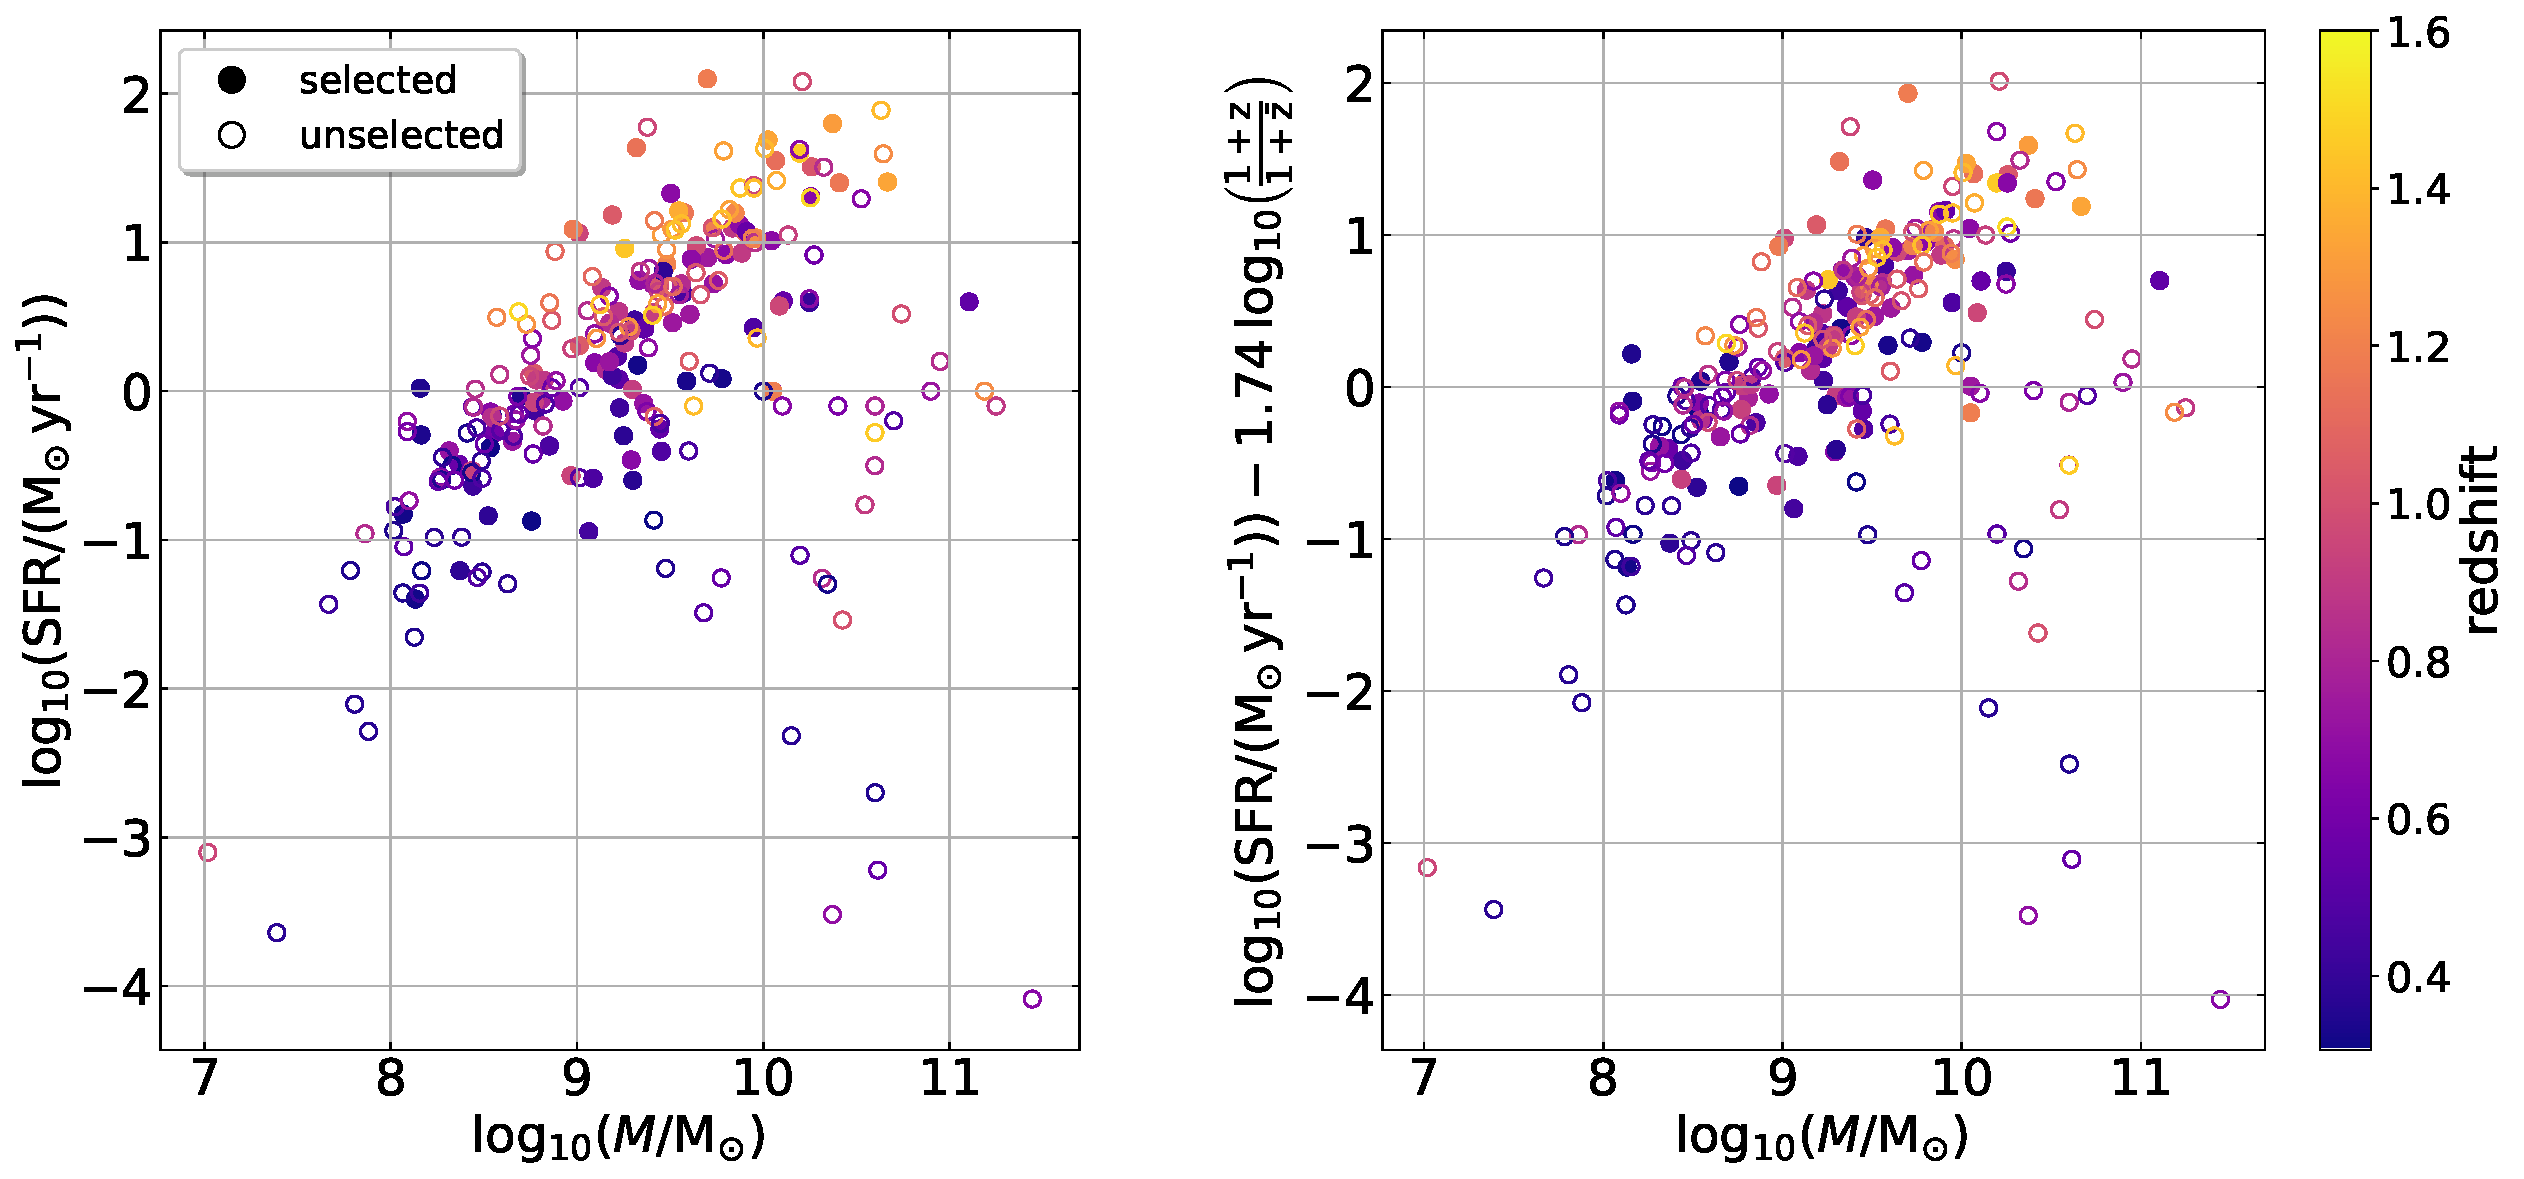
\includegraphics[width=\linewidth]{{graphics/SFR_vs_mass_withoutFAST}.pdf}
		
	\vspace{-5pt}
	\begin{itemize}[label=$\rhd$]				
		\item we recover the main sequence
		\item massive quiescent galaxies are lost
		\item redshift correction from [paper] does not improve the scatter
	\end{itemize}
\end{frame}

\section{Kinematical modelling}
\subsection{Cleaning galaxies}
\begin{frame}{Kinematical modelling}
	\framesubtitle{Cleaning galaxies}
	\begin{columns}	
		\begin{column}{0.6\linewidth}
			\vspace{100pt}		
			\centering
			
\includegraphics[width=0.5\linewidth]{{graphics/VelBefore}.eps}
		\end{column}

		\begin{column}{0.6\linewidth}
			\vspace{100pt}		
			\centering
			
\includegraphics[width=0.5\linewidth]{{graphics/VelAuto}.eps}
		\end{column}
	\end{columns}
	
	\begin{textblock*}{5cm}(8.5cm,6cm)
		
\includegraphics[width=0.6\linewidth]{{graphics/VelManual}.eps}
	\end{textblock*}
	
	%horizontal arrow and text
	\begin{textblock*}{5cm}(4.5cm,3cm)
		\centering
		\hspace{-10pt}
		Automatic \\
		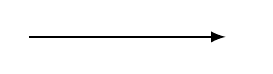
\begin{tikzpicture}[thick]
			\draw [black,   -latex      ] (0,7.0) -- (2.5,7.0) node [right] {};
		\end{tikzpicture}
	\end{textblock*}
	
	%vertical arrow
	\begin{textblock*}{5cm}(7.7cm,4.2cm)
		\centering
		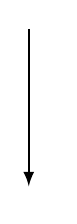
\begin{tikzpicture}[thick]
			\draw [black,   -latex      ] (0,9.0) -- (0.0,7.0) node [right] {};
		\end{tikzpicture}
	\end{textblock*}
	
	%vertical text
	\begin{textblock*}{5cm}(6.5cm,5.2cm)
		\centering
		Manual
	\end{textblock*}
	
	%three spectra
	\begin{textblock*}{7cm}(1cm,6.5cm)
		\centering
		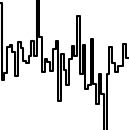
\includegraphics[width=0.25\linewidth]{{graphics/BadSpectrum}.png}
		\hfill
		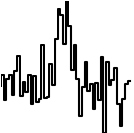
\includegraphics[width=0.25\linewidth]{{graphics/MediumSpectrum}.png}
		\hfill
		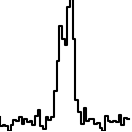
\includegraphics[width=0.25\linewidth]{{graphics/GoodSpectrum}.png}
	\end{textblock*}	
	
	%arrow for bad spectrum
	\begin{textblock*}{5cm}(-0.3cm, 4.3cm)
		\centering
		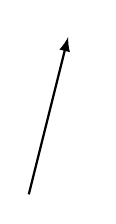
\begin{tikzpicture}[thick]
			\draw [black,   -latex      ] (0,7.0) -- (0.5,9) node [right] {};
		\end{tikzpicture}
	\end{textblock*}
	
	%arrow for medium spectrum
	\begin{textblock*}{5cm}(1cm, 3.9cm)
		\centering
		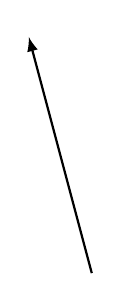
\begin{tikzpicture}[thick]
			\draw [black,   -latex      ] (0.8,7.0) -- (0,10) node [right] {};
		\end{tikzpicture}
	\end{textblock*}
	
	%arrow for medium spectrum
	\begin{textblock*}{5cm}(2.5cm, 3.3cm)
		\centering
		\begin{tikzpicture}[thick]
			\draw [black,   -latex      ] (4.5,7.0) -- (1,10.5) node [right] {};
		\end{tikzpicture}
	\end{textblock*}
	
	
\end{frame}

\subsection{Fitting a model}
\begin{frame}{Kinematical modelling}
	\framesubtitle{Fitting a model}

\end{frame}

\section{First results}
\subsection{$V_{\rm{max}}/\sigma_{\rm{v}}$ distribution}
\begin{frame}{First results}
	\framesubtitle{$V_{\rm{max}}/\sigma_{\rm{v}}$ distribution}

\end{frame}

\subsection{Tully-Fisher relation}
\begin{frame}{First results}
	\framesubtitle{Tully-Fisher relation}

\end{frame}

\section{Before you start}
\begin{frame}{Overleaf users}

\begin{alertblock}{Warning}
You can ignore this slide if you're \textbf{not} working with Overleaf.
\end{alertblock}

\vskip 0.5cm

Overleaf, Beamer and Biber do not always get along well together. For this reason, if you make a mistake while writing this presentation, in the drop-down error message you'll \textbf{always} get Biber-related error messages.

\vskip 0.5cm

Luckily, you just have to click on ``\texttt{go to first error/warning}'' and the UI will scroll to the line containing your mistake.

\end{frame}

\begin{frame}[fragile]
\frametitle{Compiling}

\begin{alertblock}{Warning}
You can ignore this slide if you \textbf{are} working with Overleaf.
\end{alertblock}

To compile this deck you'll need the \texttt{biber} package. Probably your \TeX editor already supports it; if not, you will easily find online the instructions to install it.

\vskip 0.5cm

If you're not using an editor, you can compile this presentation using the command line by running:

\begin{verbatim}
$ pdflatex main.tex
$ biber main.bcf
$ pdflatex main.tex
$ pdflatex main.tex
\end{verbatim}


\end{frame}

\section{Colors}

\begin{frame}{Colors}

For this template we defined four colors, following the graphic profile of Umeå University:
\begin{itemize}
\item \textcolor{white}{\marker[UmUBlue]{\texttt{UmUBlue}}}
\item \textcolor{white}{\marker[UmUGreen]{\texttt{UmUGreen}}}
\item \textcolor{white}{\marker[UmUPink]{\texttt{UmUPink}}}
\item \textcolor{white}{\marker[UmUGold]{\texttt{UmUGold}}}
\end{itemize}

\vskip 0.5cm

You can use these colors as you want in your presentation. For example, you can \textbf{\textcolor{UmUGold}{color the text in gold}} by writing \texttt{\textbackslash\{UmUGold\}\{my gold text\}}.

\vskip 0.5cm

We also redefined many of the most common \LaTeX{} and Beamer commands, like \texttt{itemize}, \texttt{block}, etc. You will see samples of these commands in the following slides.

\end{frame}

\section{Blocks}

\begin{frame} 
\frametitle{This is a page with a title and a subtitle} 
\framesubtitle{And also some blocks.} 
\begin{block}{Goal of the mission}
Shoot in the Death Star's exhaust port and destroy it before it can fire on the Rebel base.
\end{block} 
\begin{alertblock}{Take care!}
TIE Fighters may chase you while approaching the target.
\end{alertblock} 
\begin{exampleblock}{Use the force you must}
Remember your training with Obi-Wan, and use the Force to make the perfect shot.
\end{exampleblock} 

\end{frame}


\subsection{Description}

\begin{frame}[fragile]
\frametitle{Description}
This is an example of \texttt{description}.

\begin{description}
\item<2->[Vader] \emph{I am} your father.
\item<1->[Luke] No. No! That's not true! \textbf{That's impossible!}
\end{description}

\begin{uncoverenv}<3>
  \vskip 0.5cm
  And while we're here, let's have a look to \texttt{verbatim} as well, to see how we made items appear in arbitrary order:
  \vskip 0.5cm
  \begin{verbatim}
\begin{description}
  \item<2->[This is the first item] one
  \item<1->[This is the second item] two
\end{description}
  \end{verbatim}
\end{uncoverenv}

\end{frame}

\section{Maths}

\begin{frame}{Maths}
A formula will look like this: 
\begin{center}
 $x^2 + y^2 = z^2$
\end{center}

You can number equations as well:
\begin{equation}
1+1=2
\end{equation}

\begin{equation}
1+1=2 \tag{custom label!}
\end{equation}

\vskip 0.5cm

If you want to use the default \LaTeX{} math fonts, just go to \texttt{beamerfontthemeumu.sty} and uncomment the line containing `\texttt{\textbackslash usefonttheme[onlymath]\{serif\}}'.

\end{frame}

\begin{frame}{Theorems}

The usual \texttt{theorem}, \texttt{corollary}, \texttt{definition}, \texttt{definitions}, \texttt{fact}, \texttt{example} and \texttt{examples} blocks are available as well.

\begin{theorem}
There exists an infinite set.
\end{theorem}
\begin{proof}
This follows from the axiom of infinity.
\end{proof}
\begin{example}[Natural Numbers]
The set of natural numbers is infinite.
\end{example}

\end{frame}

\section{Other blocks}

\begin{frame}{Other blocks}

Here we display examples of \texttt{abstract}, \texttt{verse}, \texttt{quotation}, and \texttt{quote}.

\vskip 0.5cm

\begin{abstract}
This is an abstract.
\end{abstract}
\begin{verse}
This is a verse.
\end{verse}
\begin{quotation}
This is a quotation.

\raggedleft -Han Solo
\end{quotation}
\begin{quote}
A quote this is.

\raggedleft -Yoda
\end{quote}

\end{frame}

\section{Bibliography and Publications}
\begin{frame}[fragile]
\frametitle{Bibliography}

You can cite an article
\begin{itemize}
\item normally using \texttt{\textbackslash cite}, e.g.: (\cite{article1})
\item or display the full citation using \texttt{\textbackslash fullcite}, e.g.:  \fullcite{article1} \\\vspace{0.4cm}

\textit{(n.d.) stands for "no date". \texttt{year=\{A long time ago...\}} is not a date that can be specified in \texttt{bibliography} anyway.}
\end{itemize}

\vskip 0.5cm
Look at the code of the following slide to see how to automatically split the bibliography on many slides. You can also use \texttt{\textbackslash nocite\{*\}} to display the non-cited publications as well.

\end{frame}

\begin{frame}[t,allowframebreaks]
\frametitle{Bibliography}

\nocite{*} % will display the non-cited publications as well. Useful for a publication list.

\printbibliography

\end{frame}

\section{Bonus Commands}

\begin{frame}[fragile]
\frametitle{Framecard}

You can display a frame with a colored background and a huge text in the center using the command \texttt{\textbackslash framecard}.
\vskip 0.5cm 
For example, you can write:
\begin{verbatim}
\framecard{A SECTION\\TITLE}
\end{verbatim}

This will display a frame with a orange background and the phrase "A SECTION TITTLE" in the center. You can also use a custom color with \texttt{\textbackslash framecard}:
\begin{verbatim}
\framecard{A SECTION\\TITLE}
\framecard[UmUGreen]{A SECTION TITLE\\
WITH A CUSTOM COLOR}
\end{verbatim}
You can see the results of the commands above in the following slides.

\end{frame}

\framecard{A SECTION \\\vspace{3pt} TITLE}
\framecard[UmUGreen]{A SECTION TITLE\\\vspace{3pt}WITH A CUSTOM COLOR}

\begin{frame}[fragile]
\frametitle{Framepic}

You can display a frame with a background image using the command \texttt{\textbackslash framepic}. The image will be \textbf{adapted vertically} to fit the the frame. 

For example, you can write:
\begin{verbatim}
\framepic{graphics/darth}{
	\framefill
    \textcolor{white}{Luke,\\I am your supervisor}
    \vskip 0.5cm
}
\end{verbatim}

Alternatively, to make the background 50\% transparent, you can write \texttt{\textbackslash framepic[0.5]\{graphics/darth\}...}


You can see the results of the commands above in the following slides.

\end{frame}


\framepic{graphics/darth}{
	\framefill
    \textcolor{white}{Luke,\\I am your supervisor}
    \vskip 0.5cm
}

\framepic[0.5]{graphics/darth}{
	\vfill
    \begin{flushright}
    \textcolor{red}{\textbf{Right-aligned text with\\Semi-transparent background}}
    \end{flushright}	
}

\begin{frame}[t,fragile,allowframebreaks]
\frametitle{Other bonus commands}

We provide two other bonus commands:
\begin{description}
\item[\texttt{pdfnewline}] you can use \texttt{\textbackslash pdfnewline} to avoid the annoying \texttt{hyperref} related warnings when using newlines in the document's title, author, etc. For example, in this presentation the author is defined as:
\begin{verbatim}
\author[Luke Skywalker]{
  Luke Skywalker, Ph.D.
  \pdfnewline
  \texttt{luke.skywalker@uniud.it}
}
\end{verbatim}
\item[\texttt{marker}] you can use \texttt{\textbackslash marker} to highlight some text. The default color is \marker{pink}, but you can also \marker[UmUGold]{use a custom color}. For example:
\begin{verbatim}
\marker{Default color}
\marker[UmUGold]{Custom Color}
\end{verbatim}
\item[\texttt{framefill}] you can use \texttt{\textbackslash framefill} to put the text at the bottom of a slide by filling all the vertical space.
\end{description}

\end{frame}

\end{document}